\section{Dataset}
\label{sec:dataset}
\subsection{Data Composition and Reduction}
\begin{table}[h]
\centering
%Overall
%Twitter 647
%FB 21190
%FB(Other) 23098
%SMS 42551
\caption{Dataset Composition by Message Type}
\begin{tabular}{| c | c |}
\hline
\textbf{Data Type} & \textbf{Count} \\
\hline
SMS & 42551\\
\hline
Facebook & 21190\\
\hline
Facebook(Other) & 23098\\
\hline
Twitter & 647\\
\hline
\end{tabular}
\label{table:datasetCompositionMsgT}
\end{table}

We collect data from three sources \emph{viz.} SMS, Facebook \cite{facebook2016}, and Twitter \cite{twitter2016}. 
Facebook offers the most diverse data when compared with the other sources, we collect messages, likes, comments, and status updates for each participant using this platform. 
We divide the Facebook data into two parts \emph{viz.} messages (referred to as Facebook, henceforth), and a group consisting of likes, status updates, and comments (referred to as Facebook (Other), henceforth). 
Overall we obtained 87486 data points (see Table \ref{table:datasetCompositionMsgT}), where the largest share was from SMS (48.6\%), followed by Facebook (Other) (26.4\%), Facebook (24.2\%), and Twitter (0.7\%). 

\begin{table}[h]
\centering
\caption{Distribution of people during the study}
\begin{tabular}{| c | c | c |}
\hline
\textbf{Data Type} & \textbf{Participant} & \textbf{Non-Participants}\\
\hline
Overall & 69 & 932\\
\hline
SMS & 42 & 447\\
\hline
Facebook & 41 & 485\\
\hline
\end{tabular}
\label{table:datasetPvNP}
\end{table}

For the purposes of this work we only consider the SMS and Facebook data, and ignore the data from Twitter and Facebook (Other). 
This reduced dataset covers 72.8\% of the original dataset. 
There are 69 participants, and 932 non-participants in this reduced dataset (see Table \ref{table:datasetPvNP}. 
The SMS portion consists of 42 participants, and 447 non-participants, while the Facebook portion consists of 41 participants, and 485 non-participants. 
Since there could be participants who use both SMS, and Facebook to communicate with their peers, the participant counts of SMS and Facebook do not add up to the participant count of the overall (reduced) dataset. 
\begin{table}[h]
\centering
\caption{Distribution of polarity}
\begin{tabular}{| c | c | c | c | c |}
\hline
\textbf{Data Type} & \textbf{$+$} & \textbf{$-$} & \textbf{$\eta$} & $\rho$\\
\hline
Overall & 9886 & 7681 & 46174 & 1.28\\
\hline
SMS & 7114 & 4653 & 30784 & 1.53\\
\hline
Facebook & 2772 & 3028 & 15390 & 0.91\\
\hline
\end{tabular}
\label{table:polarityDist}
\end{table}

\subsection{Polarity}
For determine structural balance, we needed to assigned polarities/sentiments to the messages exchanged. There are several off-the-shelf sentiment analyzers available, and their performances differ on different datasets. 
After a search of the sentiment analyzer space we narrowed our focus to two \emph{viz.} VADER \cite{hutto2014vader}, and AFINN \cite{nielsen2011new} since both of these analyzers have been built for new-age communication media like microblogs, twitter, etc. 
Both of these tools are freely available for download and use at \cite{vader2016github, afinn2016github}. 
We randomly selected a few hundred messages and assigned them sentiment labels \emph{viz.} Positive ($+$), Negative ($-$), or Neutral ($\eta$). 
These annotations served as our ground truth. 
Next, we ran both the analyzers and evaluated their performance against the ground truth. 
Using this methodology, we found that AFINN performed significantly better than VADER on our dataset. 
AFINN was then used to assign a polarity (sentiment) to each message in our dataset. 

\begin{figure*}
\centering
\subfigure[In Degree CDF]{
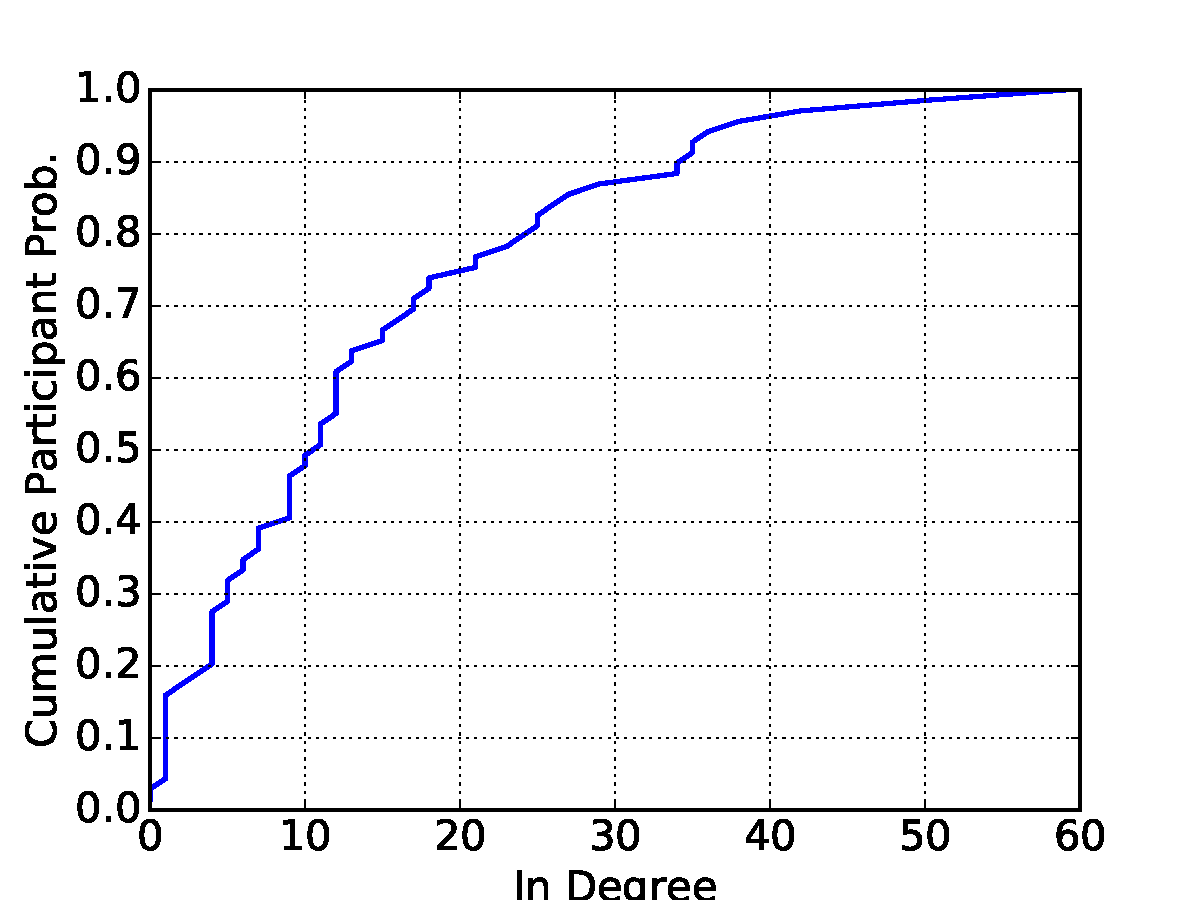
\includegraphics[width=0.22\textwidth]{in_degree.pdf}
\label{fig:inDegD}
}
\subfigure[Out Degree CDF]{
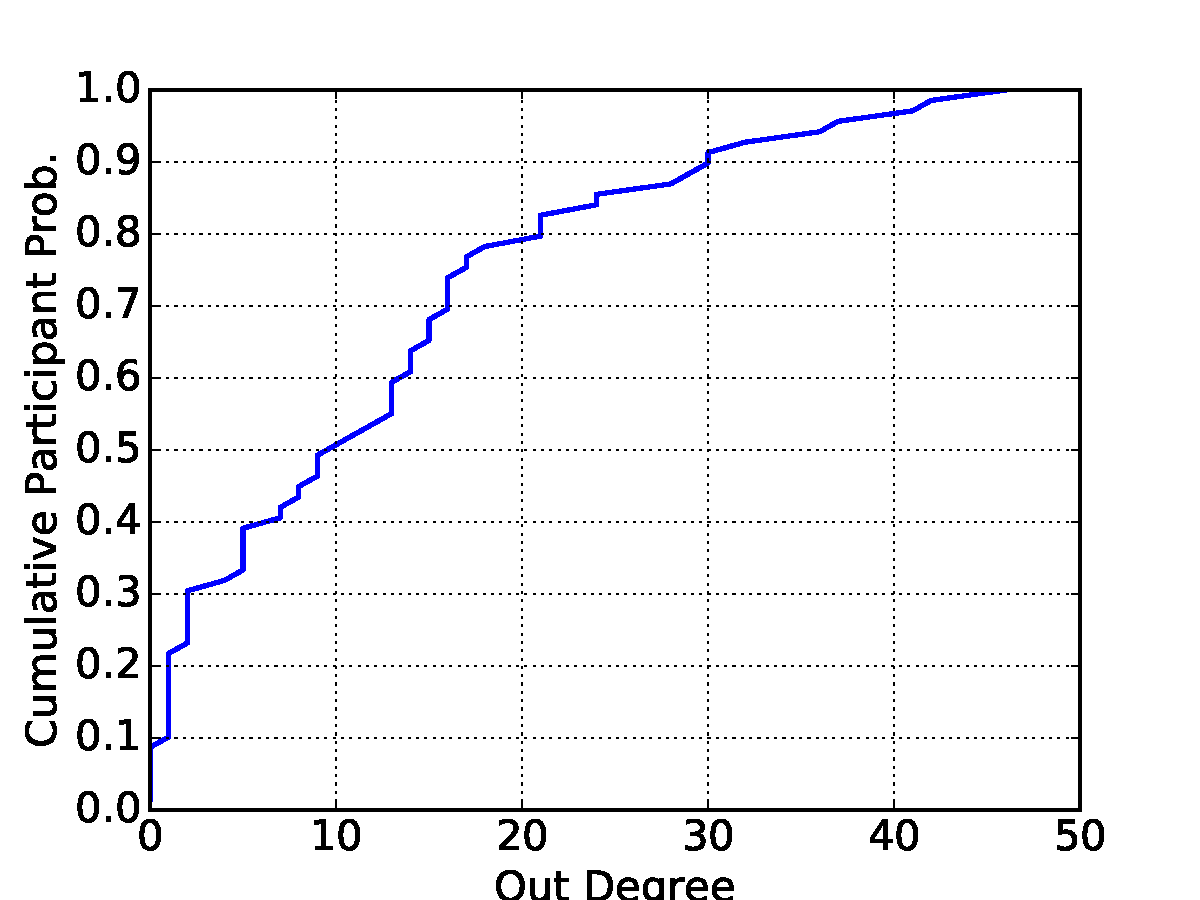
\includegraphics[width=0.22\textwidth]{out_degree.pdf}
\label{fig:outDegD}
}
\subfigure[Incoming Messages CDF]{
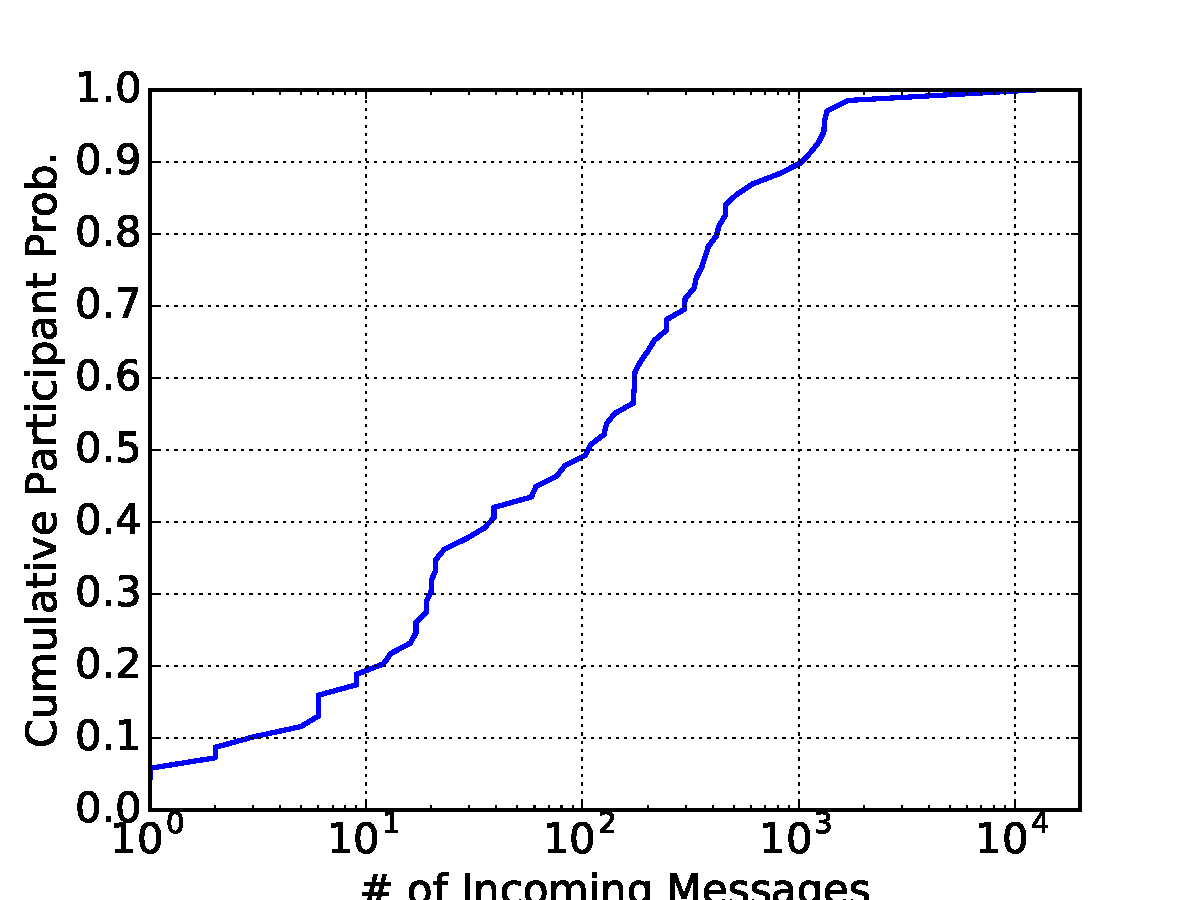
\includegraphics[width=0.22\textwidth]{in_messages.pdf}
\label{fig:inMsgD}
}
\subfigure[Outgoing Messages CDF]{
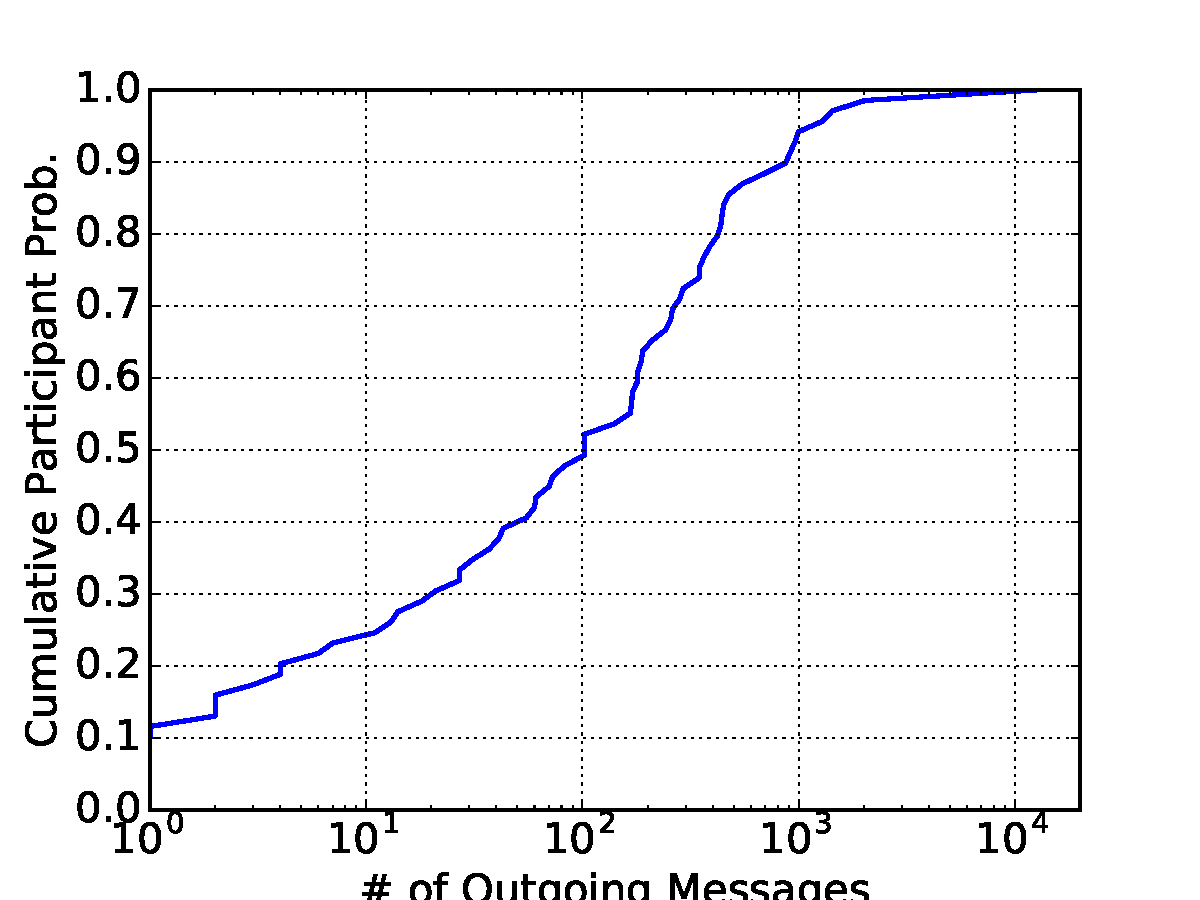
\includegraphics[width=0.22\textwidth]{out_messages.pdf}
\label{fig:outMsgD}
}
\caption{Degree and Message Distribution for the SMS+FB}
\label{fig:degMsgDist}
\end{figure*}

The polarity distribution has been summarized in Table \ref{table:polarityDist}. 
We see that neutral messages ($\eta$) dominate the dataset. 
This is expected as natural conversations are peppered with positive or negative sentiment, rather than being abundant. 
In order to see the general sentiment of the dataset we propose a new term, \emph{positivity} ($\rho$), which is the ratio of the total number of positive messages to the total number of negative messages. 
Positivity, intuitively, can be explained as the number of positive messages exchanged for each negative message. 
So, values of $\rho > 1$ indicate that the conversations tend towards positive sentiments while $\rho < 1$ indicates the tendency towards negative sentiments (or higher negativity). An ambivalent tendency is indicated by $\rho = 1$
On exploration of the SMS dataset we observe that it tends towards higher positivity while the Facebook dataset tends towards higher negativity (or lower positivity). 
These two effects counterbalance each other in the overall dataset to achieve a moderately high positivity value of 1.28. 

\subsection{Network Properties}
Here we list the properties of the network when considered across the whole duration of the study for all the participants. 
Due to the lack of complete data for the non-participants, we only concentrate on evaluating the network from a participant perspective. 
Figure \ref{fig:degMsgDist} shows the distribution of degrees (Fig. \ref{fig:inDegD}, \ref{fig:outDegD}), and the distribution of the messages (Fig \ref{fig:inMsgD}, \ref{fig:outMsgD}). 
Table \ref{table:degMsgMeanStd} shows the mean, and standard deviation of the degrees, and messages across the full duration of the study for participants. 

\begin{table}[h]
\centering
\caption{Overall Summary of Degrees and Messages for Participants}
\begin{tabular}{| c | c | c |}
\hline
 & \textbf{Mean} & \textbf{Std. Dev.}\\
\hline
In-Degree & 14.06 & 12.89\\
\hline
Out-Degree & 12.42 & 11.66\\
\hline
In-Messages & 441.27 & 1481.56\\
\hline
Out-Messages & 431.75 & 1504.43\\
\hline
\end{tabular}
\label{table:degMsgMeanStd}
\end{table}

We observe that half of the participants have 10 or less unique incoming, and outgoing degrees (edges, or connections). 
While almost all ($\approx 90\%$) have less than 35 unique incoming, and 30 unique outgoing degrees (edges, or connections). 
This suggests that most of the participants are connected to a small number of members (participants+non-participants) of the network, while only a very few have connected to a significant number of members. 
The low average in, and out degrees also corroborate this effect. 
On exploring the distribution of messages we see that half of the participants have less than 100 incoming, and outgoing messages for the whole duration of the study, while 90\% have less than 1000. 
Across the duration of the study, the participants receive 441.27 messages, and sends 431.75 messages on average which ranslates to $\approx$ 2.45 incoming, and 2.39 outgoing messages per day. 
This suggests that, on average, our participant population does not communicate highly on the different social media platforms that we collected data from.